\begin{jointwork}
	This thesis builds upon the bachelor's project `Online Marketplace Simulation: A Testbed for Self-Learning Agents' of the Enterprise Platform and Integration Concepts research group at the Hasso-Plattner-Institute. Therefore, the project will be referenced and all examples and experiments will have been conducted using its framework.
\end{jointwork}\todo{Alex: `Klassendiagramm/ FMC-Diagramm für die Übersicht? Du nennst recht Häufig Komponenten, eine Gesamtübersicht wie sie interagieren wäre gar nicht schlecht.'}

\section*{1.1\space\space Objective of the Thesis}

This thesis introduces ways to monitor and evaluate different agents (Rule-Based as well as trained using various Reinforcement-Learning approaches) tasked with dynamically pricing products in a \emph{Circular Economy} marketplace.
% Since the terms \emph{Reliability} and \emph{Robustness} can be interpreted differently depending on context and personal experience, we will define our usage in the \nameref{subsec:ReliabilityAndRobustness} section. Following the term definitions, we will give a short introduction and explanation of what a Circular Economy market is (\nameref{sec:CircularEconomy}) as well as what Reinforcement-Learning is and how we employ the technique in our framework (\nameref{sec:ReinforcementLearningIntroduction}).
We will first introduce the general concept of a \emph{recommerce} market (\nameref{sec:CircularEconomy}) and the structure of the framework we built (\todo{nameref in intro, where the diagram will be}). In \fullref{ch:RelatedWork} we will explore other aproaches to market simulations for dynamic pricing, the general concept of Reinforcement-Learning as well as novel approaches to evaluating those agents. This will be followed by an overview of the specific features of a \emph{recommerce} market that we implemented in \fullref{ch:SimulatingMarketplace}. In \fullref{ch:Approaches} we will give a detailed explanation of the different tools we built and used to monitor and evaluate our different agents. These tools will be put into context in \fullref{ch:OurWorkflow}, where the different parts of the framework will be joined together and its modularity is highlighted\todo{Highlight modularity in that chapter}. Finally, we will conduct a number of experiments using our tools in \fullref{ch:AnalyzingGraphs}.

% \subsection*{Reliability and Robustness}\label{subsec:ReliabilityAndRobustness}
% \todo{Alex: `Hast du für Reliability und Robustness irgendeine Quantifizierung? Wenn ja, und wenn die Erklärung kompakt ist würde ich die hier schon bringen.' Quantifizierung der Begriffe: Welche Metriken kommen zum Einsatz, um die jeweils zu beurteilen? Warum?}
% \begin{enumerate}
% 	\item \emph{Reliability}: With \emph{Reliability}, we describe the ability of an agent to be able to transfer knowledge of a certain type of marketplace and/or against a certain opponent over to a different scenario. If Agent A performs well against Agent B on marketplace M, does it perform the same against Agent C on marketplace M, or against Agent B on marketplace N?
% 	\item \emph{Robustness}: \emph{Robustness} is the property that describes how well an agent performs over a longer period of time. In a real-world marketplace, consistency is key to success, so finding profitability outliers and their causes are a central part of evaluating an agent's Robustness.
% \end{enumerate}

\section*{1.2\space\space The Circular Economy model}\label{sec:CircularEconomy}

The main goal of the aforementioned bachelor's project was to develop an online marketplace that simulates a realistic Circular Economy market environment. A market is most commonly referred to as being a \emph{Circular Economy} if it includes the three activities of reduce, reuse and recycle \cite{circularEconomyDefinition}. This means that while in a classical Linear Economy market each product is being sold once at its \emph{new price} and after use being thrown away, in a Circular Economy, a focus is put on recycling and thereby waste reduction. In our project, we first started by modelling the simpler Linear Economy, upon which we then built the more complex Circular Economy markets. This was done by adding two additional price channels, \emph{re-buy price} and \emph{used price}, to the pre-existing \emph{new price} of a product. Refer to \Cref{fig:IntroMarketDynamics} for an overview of the product lifecycle in a Circular economy.

\begin{figure}[t]
	\centering
	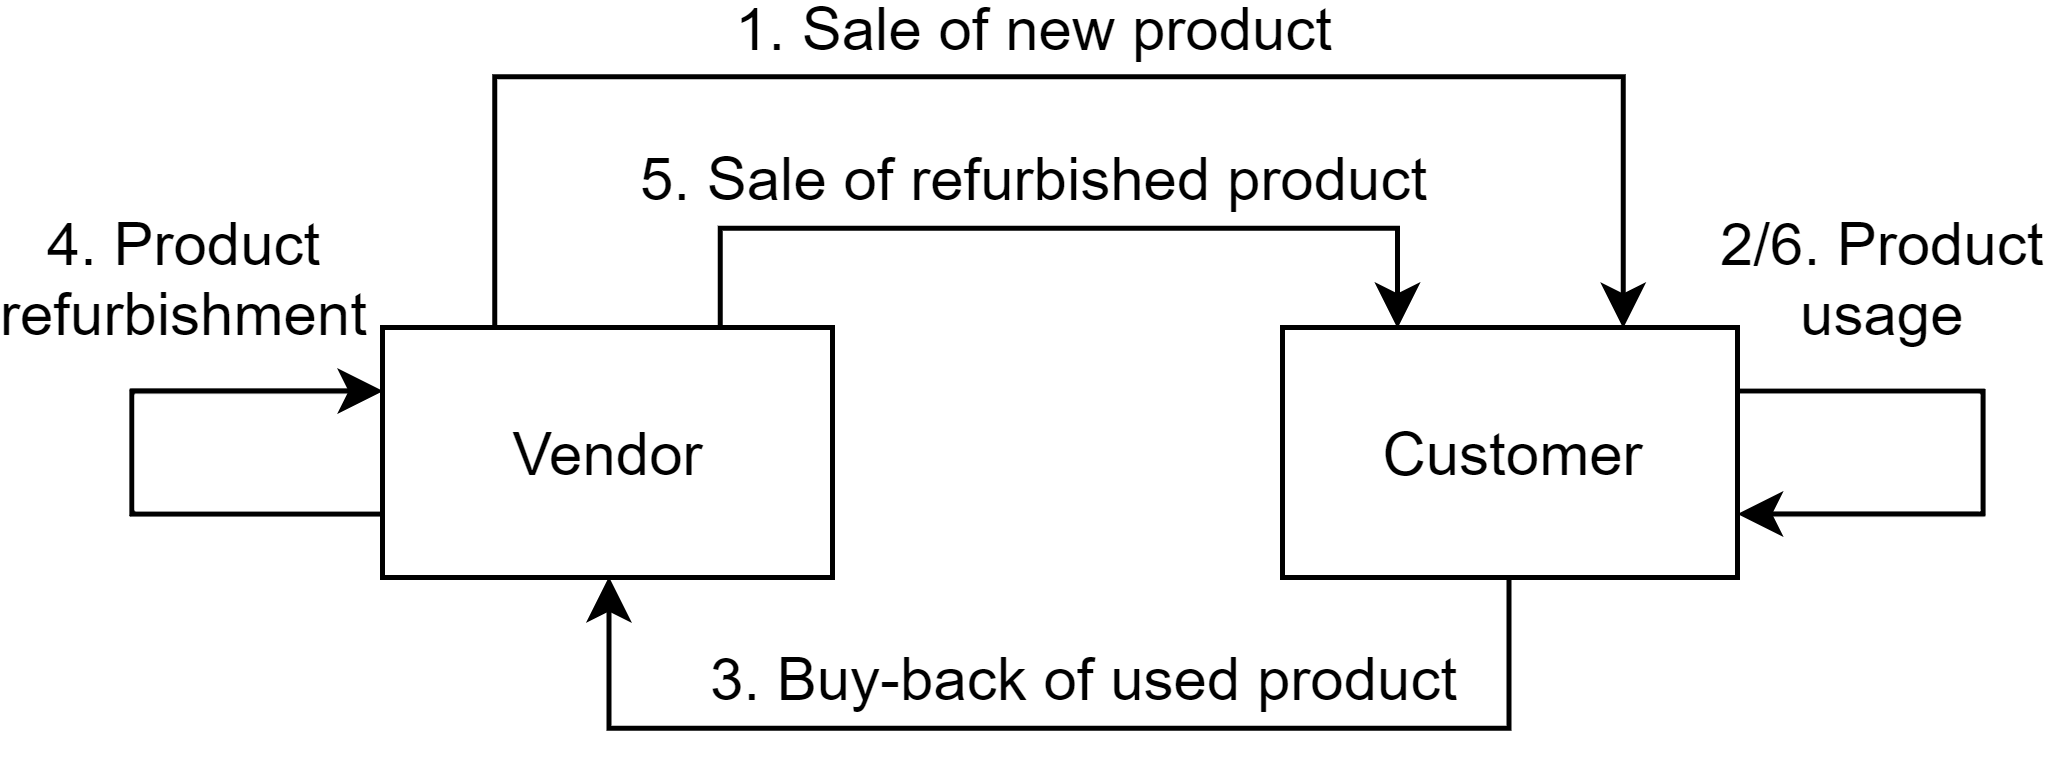
\includegraphics[width = \textwidth]{images/product_lifecycle.png}\\
	\caption{The product lifecycle in a Circular Economy. In a Linear Economy, the product lifecycle ends with step No. 2.}\label{fig:IntroMarketDynamics}
\end{figure}

The \emph{re-buy price} is defined as the price a vendor is willing to pay a customer to buy back a used product, while the \emph{used price} is defined as the price the vendor sets for products they previously bought back and now want to sell alongside new products (whose price is defined by the \emph{new price}). We will go into more detail of how we modelled different market scenarios in \nameref{sec:MarketScenarios}.

In the context of e-commerce, Circular Economy markets are also referred to as \emph{recommerce} markets. From now on, when mentioning a general \emph{market} or \emph{marketplace}, we are referencing a Circular Economy marketplace with re-buy prices.

\section*{1.3\space\space Reinforcement-Learning}\label{sec:ReinforcementLearningIntroduction}

After the initial market was modelled the goal was to train agents using different Reinforcement-Learning algorithms to dynamically set prices on this marketplace, both in monopolistic scenarios as well as in competition with Rule-Based vendors which set prices following a strict set of pre-defined rules. These rules can range from simply undercutting the lowest competitor's price to more advanced techniques such as smart inventory management and reliance on previous sales data. An overview of the different types of vendors, both Rule-Based and using Reinforcement-Learning can be found in \nameref{sec:ExplainVendors}. Furthermore, functionality was added that allows for different Reinforcement-Learning algorithms to be trained against each other on the same marketplace, as well as functionality for so-called \emph{self-play}, where an agent plays against itself, or more precisely, against its own policy.

Reinforcement-Learning agents are trained through a process of trial-and-error. They interact with the market through an observable state and an action which influences the following state. \Cref{fig:IntroRLDiagram} illustrates the RL-model in the context of our market. The goal of the agent is to maximize its \emph{reinforcement signal}, which in the case of our simulation framework is the profit the agent made during the last episode, since we want to train agents to maximize profits on real markets. An episode consists of a fixed, but pre-configurable number of timesteps, where in each step each vendor (agent) sets their prices and customers make purchasing decisions. By observing which prices lead to which profits (reinforcement signal), the agents get more effective in their pricing decisions over the course of training.

\begin{figure}[t]
	\centering
	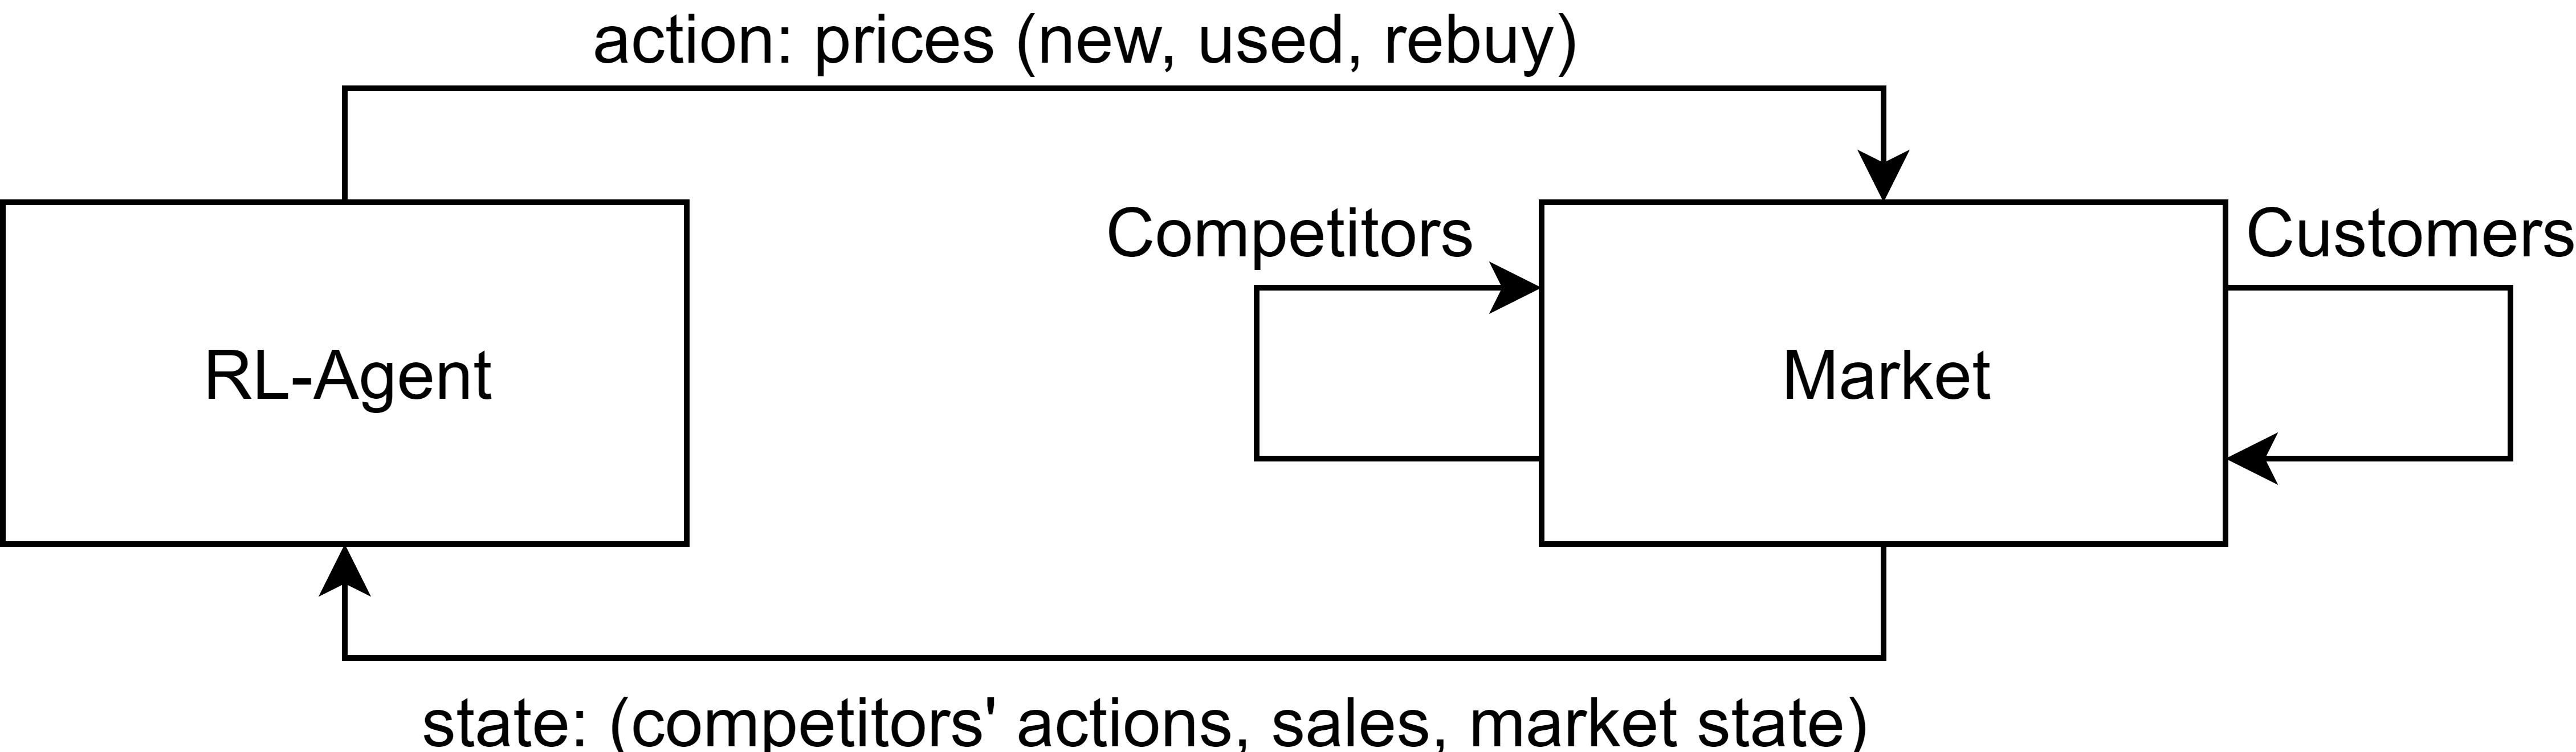
\includegraphics[width = \textwidth]{images/RL_overview.png}\\
	\caption{The standard Reinforcement-Learning model in the context of our market.}\label{fig:IntroRLDiagram}
\end{figure}